\section{General polygonal complexes by incidence geometry}
\frame{\tableofcontents[currentsection]}

\begin{frame}
    \frametitle{Motivation}
    \pause
    Goal: simplicial surfaces (and generalisations) in GAP
    \pause
    \begin{center}
                            \begin{tikzpicture}[vertexPlain=nolabels, edgeStyle=nolabels, faceStyle=nolabels]
                        % We need to define the drawing style
	
		        % First a tetrahedron
		        \begin{scope}[xshift=0cm]
			    \coordinate (A) at (0,0);
			    \coordinate (B) at (2,0);
		    	    \coordinate (C) at (0.8,1.5);
			    \coordinate (D) at (1.9,0.7);
			
                            \draw[face,edge]
                                (A) -- (B) -- (C) -- cycle
                                (B) -- (C) -- (D) -- cycle;
			    \draw[dashed,edge] (A) -- (D);
		        \end{scope}
		
		        % Second: four triangles in the form of a cone
		        \begin{scope}[xshift=3cm]
                            			    \coordinate (A) at (0,0);
			    \coordinate (B) at (1.7,0.5);
			    \coordinate (C) at (1.3,1.4);
			    \coordinate (D) at (0.5,1.5);
			    \coordinate (E) at (1,0.7);
			
			    % Take care to draw the faces in the back first
                            \draw[face,edge]
                                (A) -- (B) -- (C) -- cycle
                                (A) -- (C) -- (D) -- cycle;
                            \draw[face,edge]
                                (A) -- (B) -- (E) -- cycle
                                (A) -- (E) -- (D) -- cycle;
                            \draw[edge, dashed] (A) -- (C);

		        \end{scope}
		
		        % Three triangles that share an edge
		        \begin{scope}[xshift=7cm]
                            \coordinate (A) at (0,0);
\coordinate (B) at (0,1.5);
\coordinate (C) at (-0.7,0.4);
\coordinate (D) at (0.8,0.4);
\coordinate (E) at (0.9,0.8);
			
\draw[edge, face]
    (A) -- (B) -- (E) -- cycle;
\draw[edge,face]
    (A) -- (B) -- (C) -- cycle
    (A) -- (B) -- (D) -- cycle;
\draw[edge, dashed] (A) -- (E);
		     

		        \end{scope}
		
		        % A butterfly of triangles
		        \begin{scope}[xshift=10cm]
                            \def\LUX{-0.8}
\def\LUY{-0.3}
\def\LMX{-1.2}
\def\LMY{0.5}
\def\LOX{-0.5}
\def\LOY{1}
\coordinate (A) at (0,0);
\coordinate (B) at (\LUX,\LUY);
\coordinate (C) at (\LMX,\LMY);
\coordinate (D) at (\LOX,\LOY);
\coordinate (E) at (-\LOX,\LOY);
\coordinate (F) at (-\LMX,\LMY);
\coordinate (G) at (-\LUX,\LUY);
			
\draw[face,edge]
    (A) -- (B) -- (C) -- cycle
    (A) -- (C) -- (D) -- cycle;
\draw[faceSwap, edge]
    (A) -- (E) -- (F) -- cycle
    (A) -- (F) -- (G) -- cycle;

\foreach \p/\r/\n in {A/below/1, D/above/2, C/left/3, B/below/4, G/below/5, F/right/6, E/above/7}{
    \vertexLabelR{\p}{\r}{\n}
}

\foreach \p/\q/\n in {B/C/III, C/D/I, F/G/IV, E/F/II}{
    \node[faceLabel] at (barycentric cs:A=1,\p=1,\q=1) {\n};
}

		        \end{scope}
		
		        % An open cone of two triangles
		        \begin{scope}[xshift=1cm, yshift=-3cm]
			    \coordinate (A) at (0,0);
			    \coordinate (B) at (1.3,0.4);
			    \coordinate (C) at (0.4,1.3);
			
                            \draw[face, edge]
                                (A) -- (B) to[bend right=45] (C) -- cycle
                                (A) -- (B) to[bend left=45] (C) -- cycle;
		        \end{scope}
		
		        % A surface from non-triangular shapes
		        \begin{scope}[xshift=4cm, yshift=-3cm]
			    \coordinate (A) at (0,0);
			    \coordinate (B) at (1,0);
			    \coordinate (C) at (0.5,0.6);
			    \coordinate (D) at (0,1);
			    \coordinate (E) at (0.5,1.3);
			    \coordinate (F) at (1,1);
			    \coordinate (G) at (1.7,0.8);
			    \coordinate (H) at (1.8,0.2);
			
                            \draw[face, edge]
                                (A) -- (B) -- (C) -- cycle
                                (A) -- (C) -- (D) -- cycle
                                (D) -- (C) -- (F) -- (E) -- cycle
                                (C) -- (F) -- (G) -- (H) -- (B) -- cycle;
		        \end{scope}

                        % Double tetrahedron
                        \begin{scope}[xshift=8.7cm, yshift=-2.3cm, scale=0.5]
                            % First tetrahedron is ABCD, second one is DEFG
\coordinate (A) at (-3,-1);
\coordinate (B) at (-1,-1.5);
\coordinate (C) at (-2,1);
\coordinate (D) at (0,0);
\coordinate (E) at (3,-0.1);
\coordinate (F) at (1.5,2);
\coordinate (G) at (1.2,1);

\filldraw[face] (A) -- (B) -- (C) -- cycle;
\filldraw[face] (B) -- (C) -- (D) -- cycle;
\filldraw[faceAlt] (D) -- (F) -- (E) -- cycle;

\draw[dashed] (A) -- (D);
\draw[dashed] (E) -- (G);
\draw[dashed] (D) -- (G);
\draw[dashed] (F) -- (G);

                        \end{scope}
                    \end{tikzpicture}
 

    \end{center}
    \pause
    $\leadsto$ examples of \textbf{polygonal complexes}
\end{frame}

\begin{frame}
    \frametitle{No embedding}
    \pause
    We do \textbf{not} work with embeddings (mostly)
    \begin{itemize}
        \pause
        \item is very hard to compute \pause (compare the pentagon flippy)
        \pause
        \item if often unknown for an abstractly constructed surface
        \pause
        \item is different from \textit{intrinsic structure}
        \pause
        \item[$\Rightarrow$] lengths and angles are not important
        \pause
        \item[$\leadsto$] incidence structure is intrinsic
    \end{itemize}
\end{frame}

\begin{frame}[fragile]
    % The option is needed: https://tex.stackexchange.com/questions/119309/arguments-of-tikzset-inside-a-beamer-document
    \frametitle{Incidence structure of a polygonal complex}
    \onslide<2->{
        A \textbf{polygonal complex} consists of
    }
    
    \begin{itemize}
        \item<3-> set of vertices $\mathcal{V}$ \hfill
            \onslide<4->{
                \begin{tikzpicture}
                    \newcommand{\vertexDot}[2]{
                        % xshift, label
                        \coordinate[label={[\vertexColor]right:#2}] (V#2) at (#1,0);
                        \fill[vertex] (V#2) circle (\vSize);
                    }

                    \onslide<4-9>{
                        \vertexDot{0}{2}
                    }
                    \onslide<4-13>{
                        \vertexDot{1}{3}
                        \vertexDot{2}{5}
                    }
                    \onslide<4-14>{
                        \vertexDot{3}{7}
                    }
                    \onslide<4-19>{
                        \vertexDot{4}{11}
                    }
                \end{tikzpicture}
            }
        \item<5-> set of edges $\mathcal{E}$ \hfill
            \onslide<6->{
                {\small
                \begin{tikzpicture}[scale=0.9]
                    \newcommand{\storedEdge}[2]{
                        \coordinate (A#2) at (-0.6+#1*1.5, -0.3);
                        \coordinate (B#2) at (0.6+#1*1.5, 0.3);
                        \draw[edge] (A#2) -- (B#2);
                        \drawEdge{A#2}{B#2}{#2}
                    }

                    \onslide<6-9>{
                        \storedEdge{0}{6}
                    }
                    \onslide<6-12>{
                        \storedEdge{1}{8}
                        \storedEdge{2}{9}
                    }
                    \onslide<6-16>{
                        \storedEdge{3}{10}
                    }
                    \onslide<6-19>{
                        \storedEdge{4}{12}
                        \storedEdge{5}{13}
                    }
                \end{tikzpicture}
                }
            }
        \item<7-> set of faces $\mathcal{F}$ \hfill
            \onslide<8->{
                {\small
                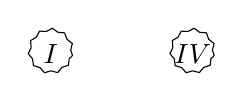
\begin{tikzpicture}[scale=0.9,
                        decoration={snake, amplitude=0.5, segment length=4.5}]
                    \onslide<8-10>{
                        \node at (0,0) {$I$};
                        \draw[decorate] (0,0) circle (0.3);
                    }
                    \onslide<8-18>{
                        \node at (2,0) {$IV$};
                        \draw[decorate] (2,0) circle (0.3);
                    }
                \end{tikzpicture}
                }
            }
        \item<9-> transitive relation \def\brSize{\big}
            $\subset \brSize(\mathcal{V} \times \mathcal{E} \brSize)
            \uplus \brSize(\mathcal{V} \times \mathcal{F} \brSize)
            \uplus \brSize(\mathcal{E} \times \mathcal{F} \brSize)$
    \end{itemize}
    % Draw the pictures
    \onslide<10->{
        \begin{tikzpicture}[vertexNode/.style={circle, draw=\vertexColor}, node distance=0.5]

            % Edge nodes
            \node[edgeBackground] (E6) {6};
            \uncover<13->{
                \node[edgeBackground] (E8) [right=of E6] {8};
                \node[edgeBackground] (E9) [right=of E8] {9};
            }
            \uncover<17->{
                \node[edgeBackground] (E10) [right=of E9] {10};
            }
            \uncover<20->{
                \node[edgeBackground] (E12) [right=of E10] {12};
                \node[edgeBackground] (E13) [right=of E12] {13};
            }

            % Face nodes
            \uncover<11->{
                \node (F1) [above=of E8] {$I$};
                \draw (F1) -- (E6);
            }
            \uncover<13->{
                \draw (E8) -- (F1);
                \draw (E9) -- (F1);
            }

            \node (Help) at ($(E10)!0.5!(E12)$) {};
            \uncover<19->{
                \node (F4) [above=of Help] {$IV$};
                \draw (F4) -- (E9);
                \draw (F4) -- (E10);
            }
            \uncover<20->{
                \draw (E12) -- (F4) -- (E13); %TODO does this look good?
            }

            % Vertex nodes
            \uncover<15->{
                \node[vertexNode] (V7) [below=of Help] {7};
            }
            \uncover<17->{
                \draw (E10) -- (V7);
            }
            \uncover<20->{
                \draw (E13) -- (V7);
            }

            \uncover<20->{
                \node[vertexNode] (V11) [right=of V7] {11}
                    edge (E13) edge (E12);
            }

            \uncover<14->{
                \node[vertexNode] (V5) [left=of V7] {5}
                    edge (E8) edge (E9);
                \node[vertexNode] (V3) [left=of V5] {3}
                    edge (E6) edge (E9);
            }
            \uncover<20->{
                \draw (E12) -- (V5);
            }
            \uncover<17->{
                \draw (E10) -- (V3);
            }

            \uncover<10->{
                \node[vertexNode] (V2) [left=of V3] {2}
                    edge (E6);
            }
            \uncover<13->{
                \draw (E8) -- (V2);
            }

            \begin{scope}[xshift=7cm, yshift=-0.6cm, scale=0.7]
                %       P3 ------------ P4
                %      / |       10     | 
                %    6/  |              |
                %    /   |              |
                %  P1  I |9      IV     |13
                %    \   |              |
                %    8\  |              |
                %      \ |        12    |
                %       P2 ------------ P5

                \uncover<10->{
                    \coordinate[label={[vertex]left:2}] (P1) at (0,0.5);
                }
                \uncover<14->{
                    \coordinate[label={[vertex]below:5}] (P2) at (2,-1);
                    \coordinate[label={[vertex]above:3}] (P3) at (2,2);
                }
                \uncover<15->{
                    \coordinate[label={[vertex]above:7}] (P4) at (5,2);
                }
                \uncover<20->{
                    \coordinate[label={[vertex]below:11}] (P5) at (5,-1);
                }

                % Draw first face
                \onslide<11-12>{
                    \fill[\faceColor] (P1) -- (P2) -- (P3) -- cycle;
                    \node at ($1/3*(P1)+1/3*(P2)+1/3*(P3)$) {I};
                }
                \onslide<13->{
                    \filldraw[face] (P1) -- (P2) -- (P3) -- cycle;
                    \node at ($1/3*(P1)+1/3*(P2)+1/3*(P3)$) {I};
                }
                \onslide<10-12>{
                    \draw[\edgeColor] (P1) -- (P3);
                }

                % Draw the second face
                \onslide<19>{
                    \fill[\faceColor] (P2) -- (P3) -- (P4) -- (P5) -- cycle;
                    \node at ($1/4*(P2)+1/4*(P3)+1/4*(P4)+1/4*(P5)$) {IV};
                }
                \onslide<17-19>{
                    \draw[\edgeColor] (P3) -- (P4);
                }
                \onslide<20->{           
                    \filldraw[face] (P2) -- (P3) -- (P4) -- (P5) -- cycle;
                    \node at ($1/4*(P2)+1/4*(P3)+1/4*(P4)+1/4*(P5)$) {IV};
                }
        

                % Draw the edges
                \onslide<10->{
                    \drawEdge{P1}{P3}{6}
                }
                \onslide<13->{
                    \drawEdge{P1}{P2}{8}
                    \drawEdge{P2}{P3}{9}
                }
                \onslide<17->{
                    \drawEdge{P3}{P4}{10}
                }
                \onslide<20->{
                    \drawEdge{P4}{P5}{13}
                    \drawEdge{P5}{P2}{12}
                }

                % Draw the concrete points
                \onslide<10->{
                    \fill[vertex] (P1) circle (\vSize);
                }
                \onslide<14->{
                    \fill[vertex] (P2) circle (\vSize);
                    \fill[vertex] (P3) circle (\vSize);
                }
                \onslide<15->{
                    \fill[vertex] (P4) circle (\vSize);
                }
                \onslide<20->{
                    \fill[vertex] (P5) circle (\vSize);
                }
            \end{scope}
        \end{tikzpicture}
    }
    \begin{enumerate}
        \item<12-> Every face is a polygon
        \item<16-> Every vertex lies in an edge \onslide<18->{and every edge lies in a face}
    \end{enumerate}
\end{frame}


\begin{frame}{Isomorphism testing}
    \pause
    Incidence geometry allows ``easy" isomorphism testing.
    \pause
    Incidence structure can be interpreted as a coloured graph:
    \pause
        \begin{center}
        \begin{tikzpicture}[vertexNode/.style={circle,
            fill=magenta!50!white}, node distance=0.5]
            % Edge nodes
            \node[edgeBackground] (E6) {6};
            \node[edgeBackground] (E8) [right=of E6] {8};
            \node[edgeBackground] (E9) [right=of E8] {9};
            \node[edgeBackground] (E10) [right=of E9] {10};
            \node[edgeBackground] (E12) [right=of E10] {12};
            \node[edgeBackground] (E13) [right=of E12] {13};

            % Face nodes
            \node[fill=yellow] (F1) [above=of E8] {$I$}
                edge (E6) edge (E8) edge (E9);
            \node (Help) at ($(E10)!0.5!(E12)$) {};
            \node[fill=yellow] (F4) [above=of Help] {$IV$}
                edge (E9) edge (E10) edge (E12) edge (E13);

            % Vertex nodes
            \node[vertexNode] (V7) [below=of Help] {7}
                edge (E10) edge (E13);
            \node[vertexNode] (V11) [right=of V7] {11}
                edge (E13) edge (E12);
            \node[vertexNode] (V5) [left=of V7] {5}
                edge (E8) edge (E9) edge (E12);
            \node[vertexNode] (V3) [left=of V5] {3}
                edge (E6) edge (E9) edge (E10);
            \node[vertexNode] (V2) [left=of V3] {2}
                edge (E6) edge (E8);
        \end{tikzpicture}
        \end{center}
    \pause
    $\leadsto$ reduce to graph isomorphism problem

    \pause
    Solved by NautyTracesInterface (by Gutsche, Niemeyer, Schweitzer)
\end{frame}


\begin{frame}{General properties}
    \pause
    Some properties can be computed for all polygonal complexes:
    \pause
    \begin{itemize}
        \item Connectivity
        \pause
        \item Euler--Characteristic
    \end{itemize}
    \pause
    \textit{Orientability} is \textbf{not} one of them.
    \pause
    Counterexample:
        \begin{center}
            \begin{tikzpicture}
                \coordinate (A) at (0,0);
                \coordinate (B) at (0,1.5);
                \coordinate (C) at (-0.7,0.4);
                \coordinate (D) at (0.8,0.4);
                \coordinate (E) at (0.9,0.8);
                			
                % draw back face first
                \filldraw[face] (A) -- (B) -- (E) -- cycle;
                % Now draw front faces
                \filldraw[face] (A) -- (B) -- (C) -- cycle;
                \filldraw[face] (A) -- (B) -- (D) -- cycle;
                % Draw dashed line
                \draw[dashed] (A) -- (E);
	    \end{tikzpicture}
        \end{center}
    \pause
    $\Rightarrow$ every edge lies in at most two faces (for well--definedness)
    
    \pause
    $\leadsto$ \textbf{ramified polygonal surfaces}
\end{frame}


\begin{frame}{Why ramified?}
    \pause
    Typical example of ramified polygonal surface:
    \pause
    \begin{center}
        \begin{tikzpicture}
                % First tetrahedron is ABCD, second one is DEFG
                \coordinate (A) at (-3,-1);
                \coordinate (B) at (-1,-1.5);
                \coordinate (C) at (-2,1);
                \coordinate (D) at (0,0);
                \coordinate (E) at (3,-0.1);
                \coordinate (F) at (1.5,2);
                \coordinate (G) at (1.2,1);
                
                \filldraw[face] (A) -- (B) -- (C) -- cycle;
                \filldraw[face] (B) -- (C) -- (D) -- cycle;
                \filldraw[faceAlt] (D) -- (F) -- (E) -- cycle;
                
                \draw[dashed] (A) -- (D);
                \draw[dashed] (E) -- (G);
                \draw[dashed] (D) -- (G);
                \draw[dashed] (F) -- (G);
        \end{tikzpicture}
    \end{center}
    \pause
    $\Rightarrow$ It is not a surface -- there is a \textit{ramification} at 
        the central vertex
    
    \pause
    A \textbf{polygonal surface} does not have these ramifications.
\end{frame}


